\section{Flow Management for Resilience}
\label{sec:resilience}

\subsection{Distributed Flow Migration}

\begin{figure}[!h]
\begin{subfigure}[t]{0.33\linewidth}
   \centering
   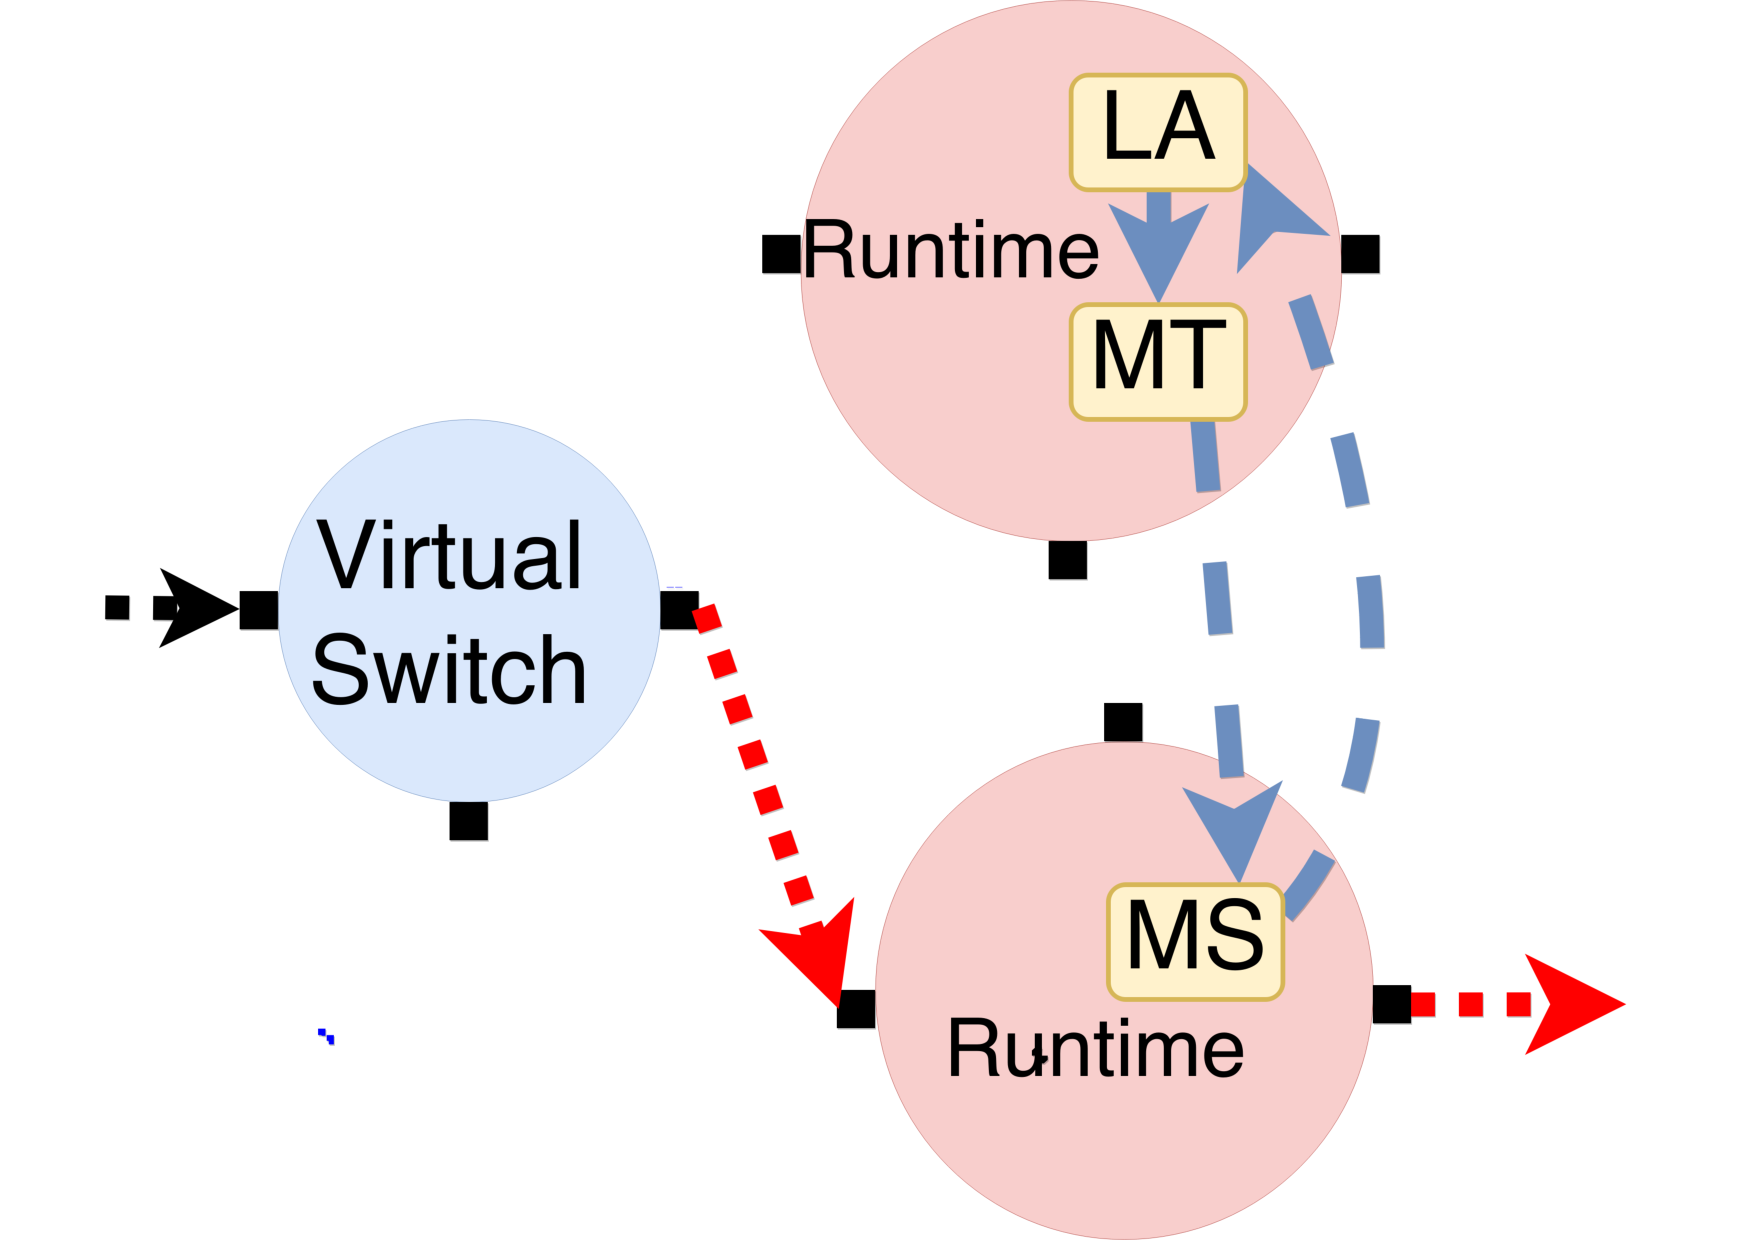
\includegraphics[width=\columnwidth]{figure/nfactor-mig1.pdf}
   \caption{1st req-rep.}\label{fig:mig1}
  \end{subfigure}\hfill
  \begin{subfigure}[t]{0.33\linewidth}
     \centering
     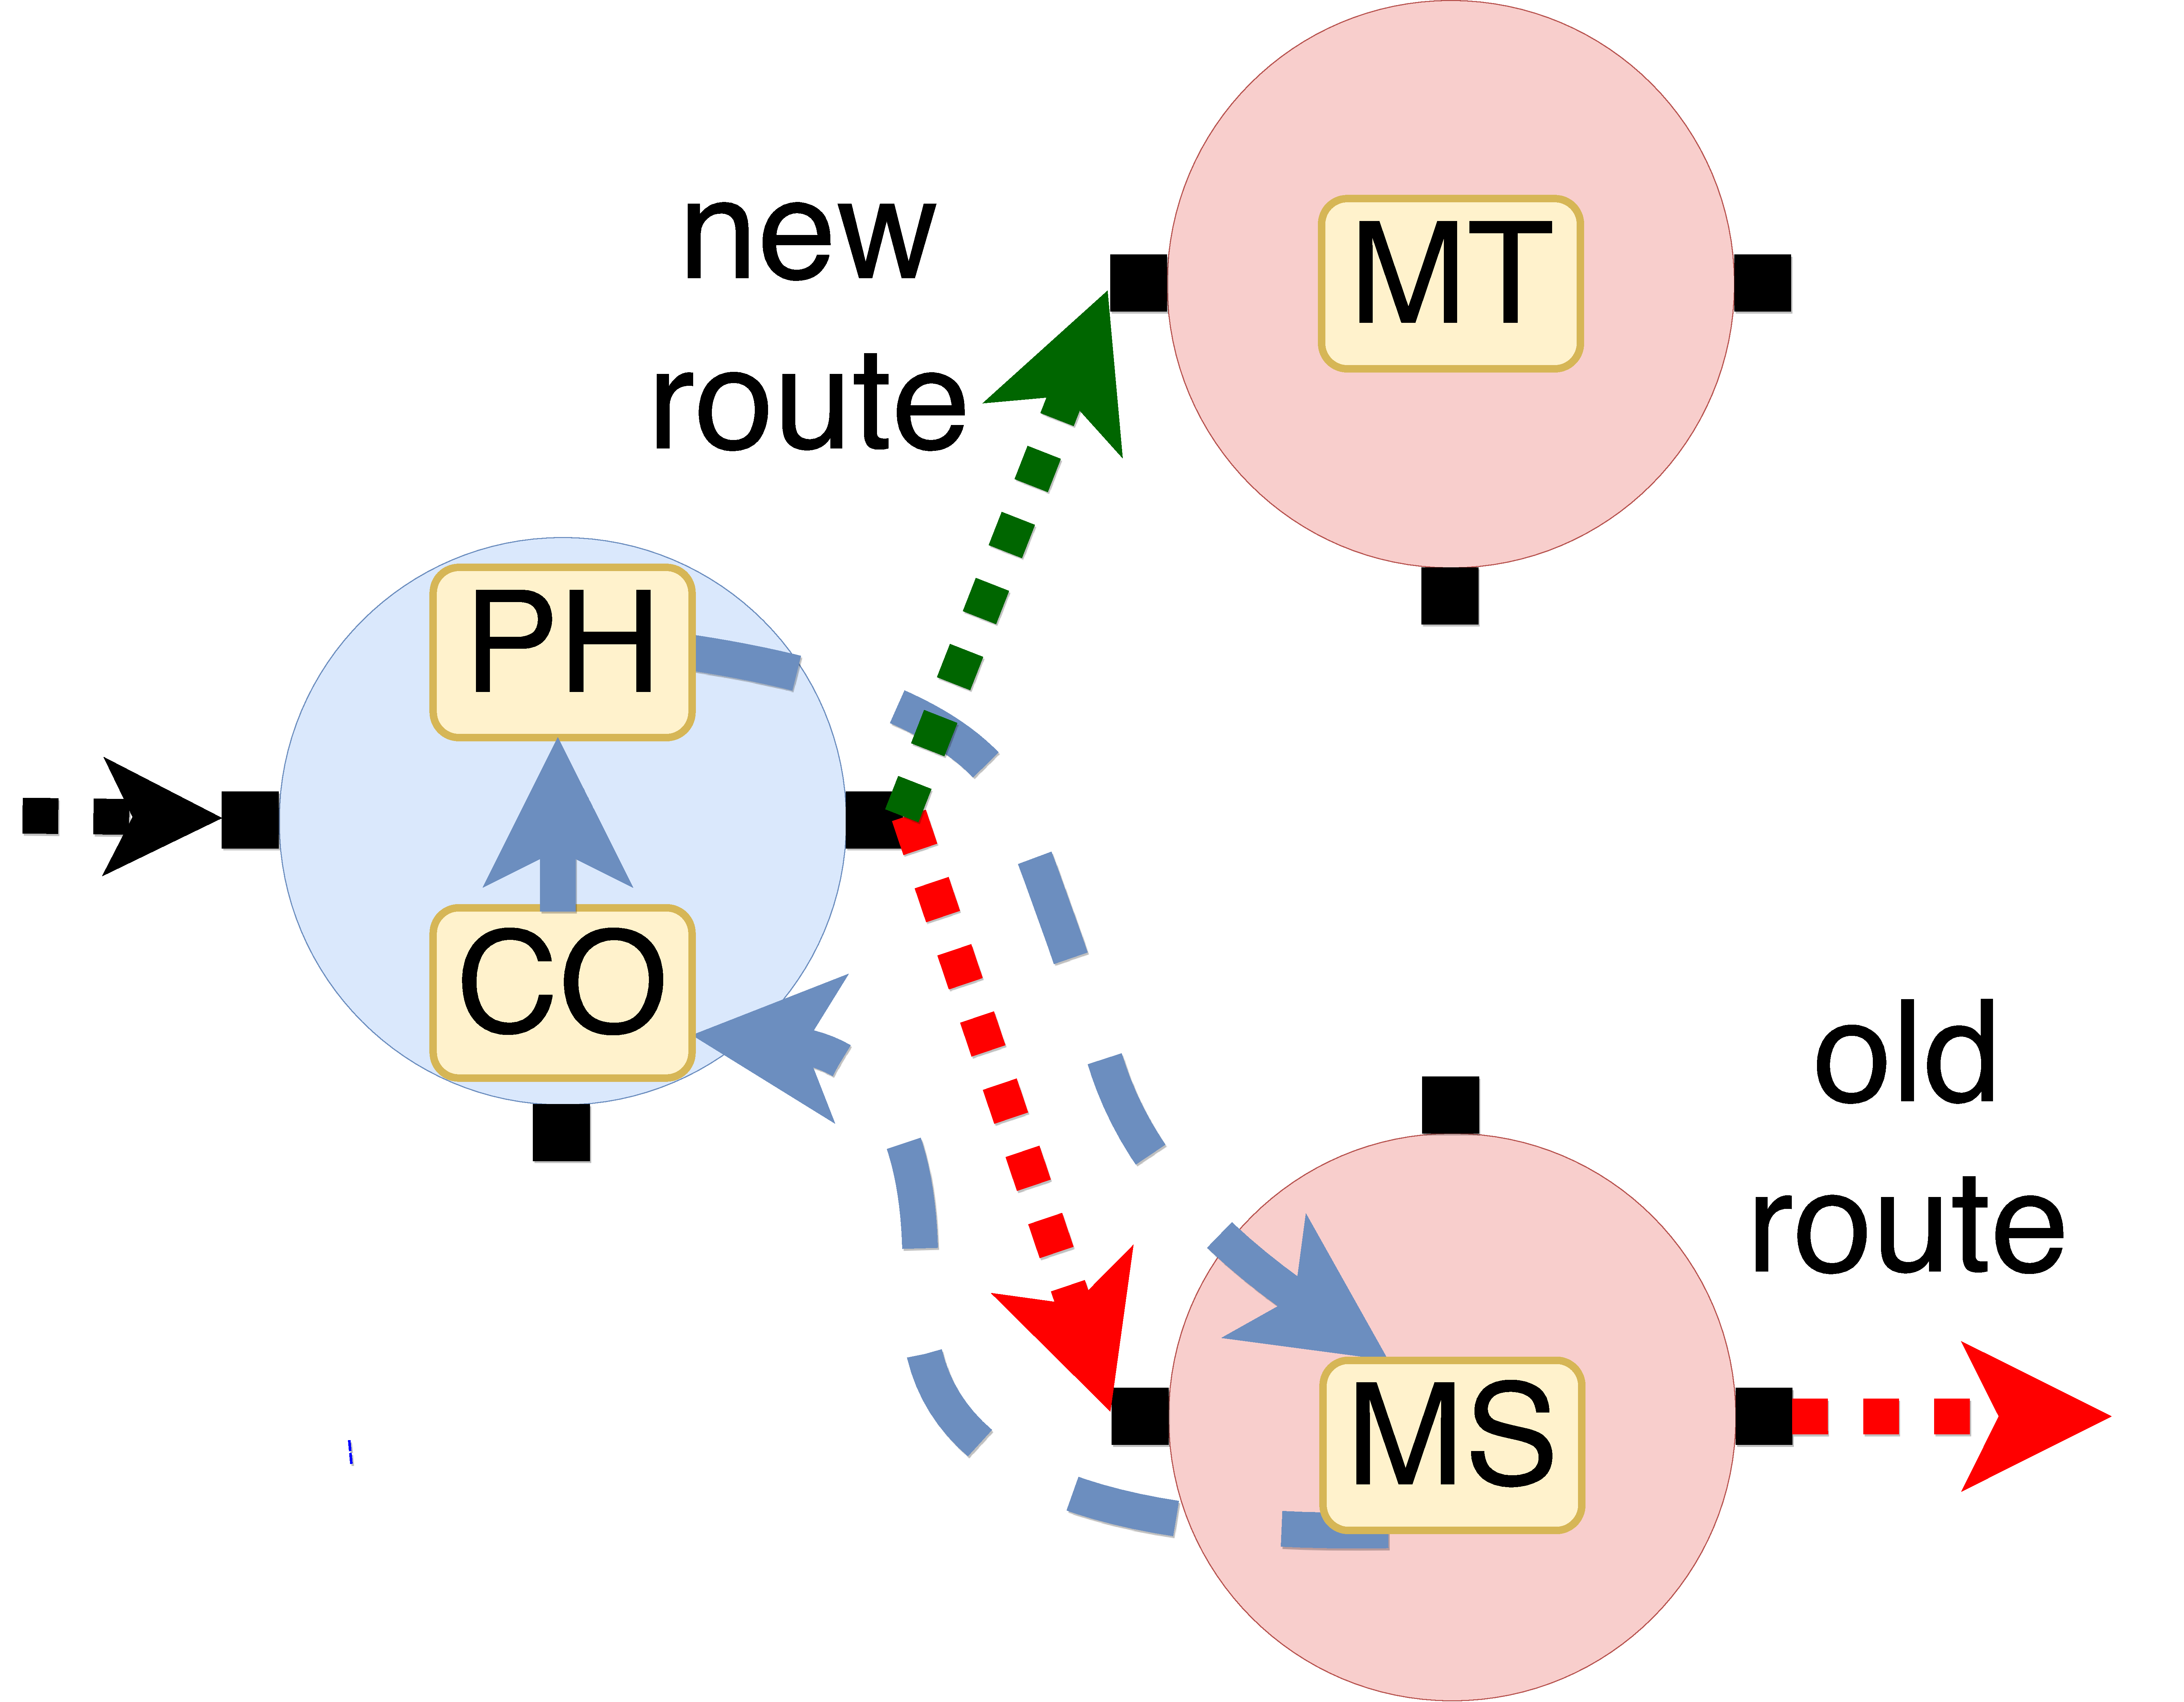
\includegraphics[width=\columnwidth]{figure/nfactor-mig2.pdf}
     \caption{2nd req-rep.}\label{fig:mig2}
    \end{subfigure}\hfill
  \begin{subfigure}[t]{0.33\linewidth}
 \centering
   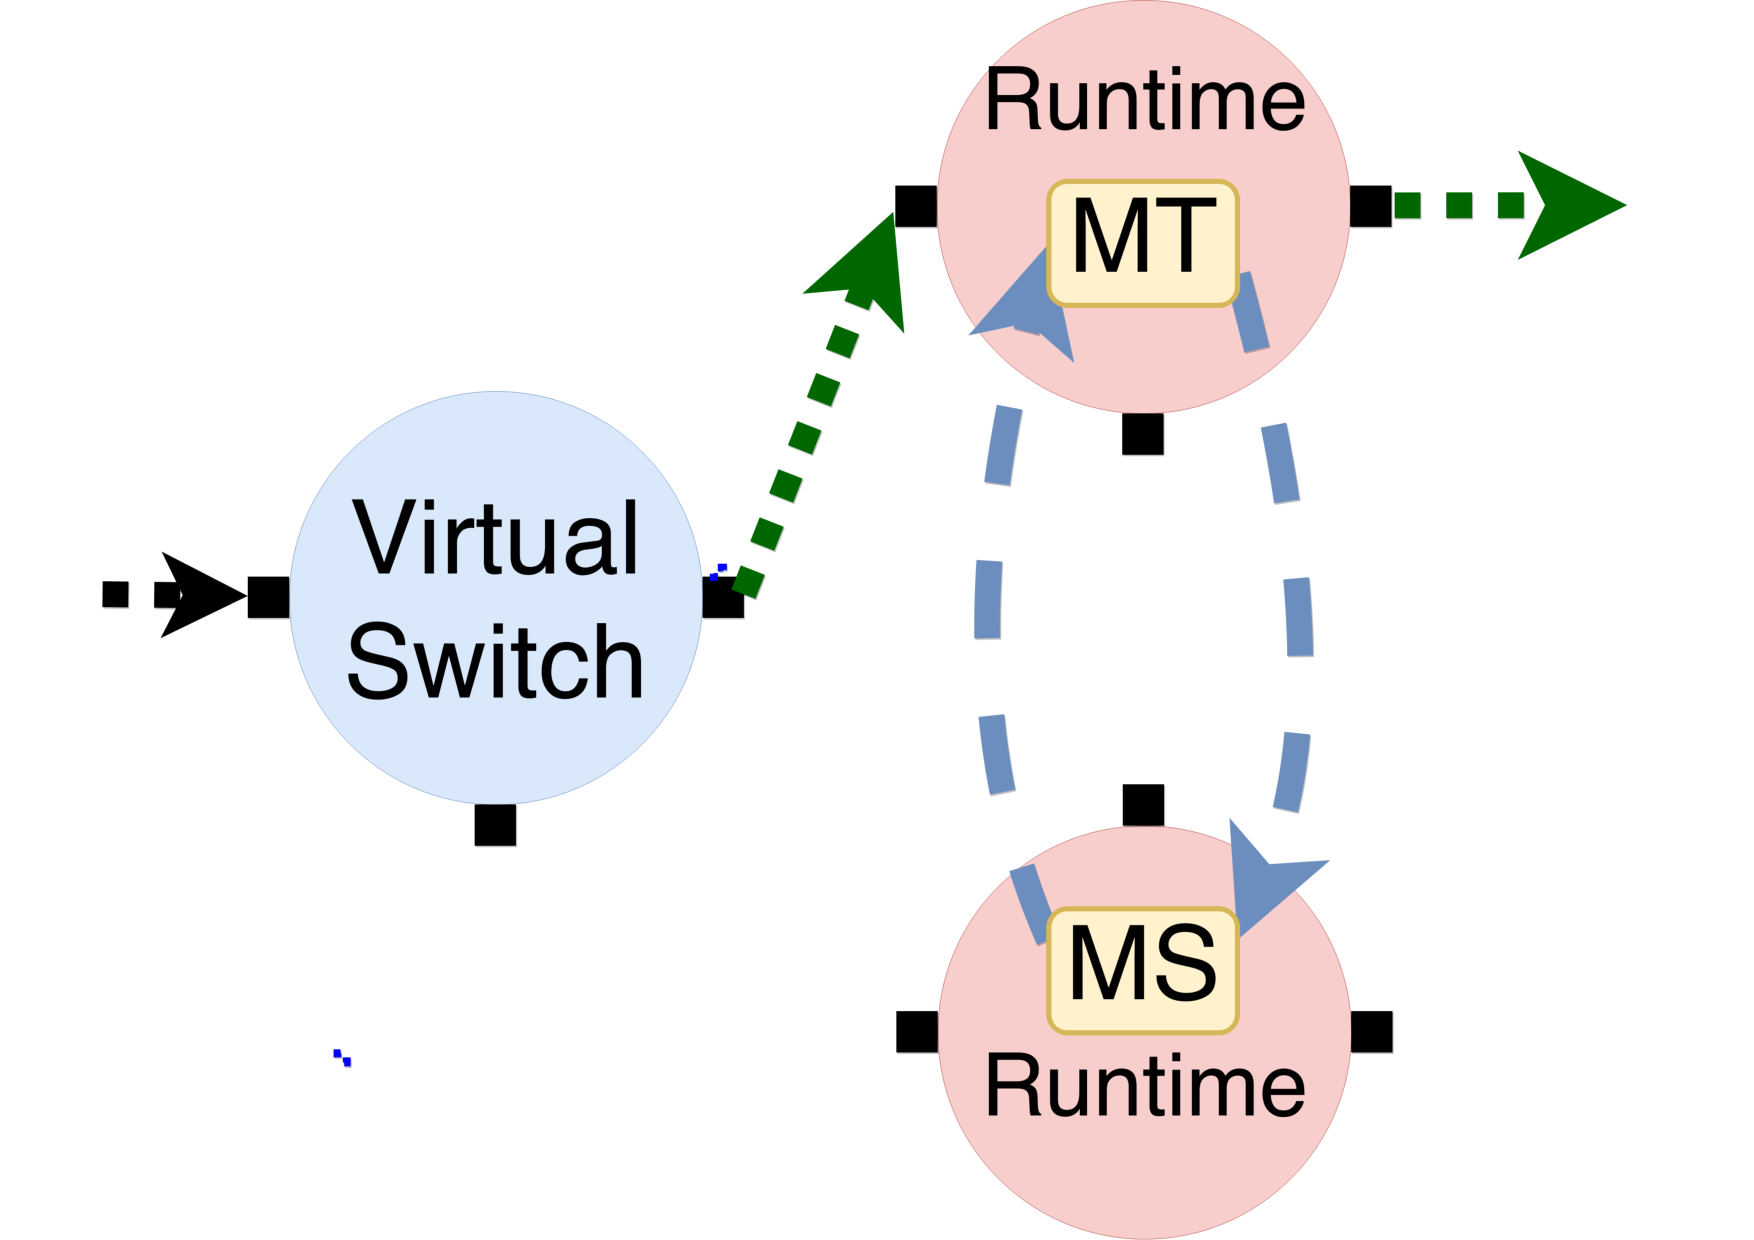
\includegraphics[width=\columnwidth]{figure/nfactor-mig3.pdf}
   \caption{3rd req-rep.}\label{fig:mig3} \end{subfigure}\hfill
 \caption{The flow migration process that migrates migration source actor running on migration source runtime to migration target runtime. (\textbf{MT}: Migration target actor. \textbf{MS}: Migration source actor. \textbf{CO}: Coordinator actor. \textbf{VS}: Virtual switch actor. \textbf{Dotted line}: Dataplane flow packets. \textbf{Dashed line}: Actor messages.)}
\label{fig:mig}
\end{figure}

Figure \ref{fig:mig} shows workflow of \nfactor's flow migration, which involves passing three request-response. Besides being fully distributed, the flow migration also guarantees two properties that (i) except for the migration target side buffer overflow or network packet reordering (which rarely happens in \nfactor), no flow packets are dropped by the flow migration protocol, which we refer to as \textbf{loss-avoidance} property (this is slightly weaker that the loss-free property in OpenNF \cite{gember2015opennf}) and (ii) the same \textbf{order-preserving} property as in OpenNF \cite{gember2015opennf}. There has been a long understanding that providing good properties for flow migration would compromise the performance of flow migration \cite{gember2015opennf}. \nfactor~ breaks this misunderstanding using the novel distributed flow migration.

Runtimes can check the received cluster view list to obtain the contact address and load information of other runtimes, and select an appropriate target for flow migration and repli- cation.

The details of the three request-responses are summarized below.
\begin{itemize}

\item \textbf{1st req-rep:} The migration source actor sends its flow-5-tuple to the coordinator actor on the migration target runtime. The coordinator actor creates a migration target actor using the flow-5-tuple contained in the request, which returns a response back to the migration source actor. During the execution of the first request-response, migration source actor continues to process packet.

\item \textbf{2nd req-rep:} The current flow actor sends its flow-5-tuple and the ID of the migration target runtime to the coordinator actor on the virtual switch. The coordinator actor uses the flow-5-tuple to find out the virtual switch actor and notifies it to change the destination runtime to migration target runtime. After changing the destination runtime, the virtual switch actor sends a response back to the migration source actor. The migration target actor starts to receive packets after the destination runtime of the virtual switch actor is changed and buffer all the received packets until it receives the third request. In the meantime, the migration source actor keeps processing the input packets until it receives the second response.

\item \textbf{3rd req-rep:} the migration source actor sends its flow state to the migration target actor. After receiving the flow states, the migration target actor saves them, gives a response to the migration source actor and immediately start processing all the buffered packets. The migration source actor exits when it receives the response.

\end{itemize}

\textbf{The Loss-Avoidance Property.} Before the migration target actor receives the third request, it needs to buffer input packets indefinitely, which might lead to a buffer overflow if the third request takes a long time to arrive. \nfactor~ simply drops additional flow packets after buffer overflow because \nfactor~ needs to process packet at a high throughput rate and does not want to grow buffer indifinitely. In \nfactor, a large collective buffer is used to buffer the packets for different migration target actors and the distributed flow migration process is extremely fast, so the buffer overflow rarely happens, even when migrating a huge number of flows. This is demonstrated in the evaluation section \ref{}.

Besides buffer overflow, the only step that might incur potential packet drop is in the third request-response. When the second response is received by the migration source actor, it must immediately send its flow state in the third request to the migration target actor. After sending the third request, there might be pending flow packets continuing to arrive at migration source actor. These pending packets are are sent out by the virtual switch actor before the destination runtime is changed. If this happens, the migration source actor has to discard these pending flow packets because it has already sent out the third request. Continuing to process these packets may generate inconsistent output packets.

If the network doesn't reorder packet, which is a common case because \nfactor~is deployed over a L2 network, \nfactor's flow migration can eliminate the second cause of packet drop by transmitting second response in a network packet over the same network path as the data plane packets that are sent to the migration source actor. Recall that in Figure \ref{fig:runtime-arch}, the remote messages could be sent over input/output port of a runtime. The second response is encapsulated in a raw packet \ref{}, sent by the output port of the virtual switch and received by the input port of the migration source runtime, therefore sharing the same network path as the data plane packets that are sent to the migration source actor.

Because the second response are sent after the destination runtime of the virtual switch actor is changed and share the same network path as the data plane packets that are sent to the migration source actor, it also becomes a strong indication that no more input packets will be sent to the migration source actor. This is verified in our evaluation \ref{}.

\textbf{Order-preserving Property.} Since the second request-response eliminate the packet drop if the network doesn't reorder packets, flow packets could always be processed in the order that they are sent out from the virtual switch. The order-preserving property is therefore guaranteed.

\textbf{Error Handling.} The three request-responses may not always be successfully executed. In case of request timeout, the migration source actor is responsible for restoring the destination runtime of the virtual switch actor (if it is changed) and resumes normal packet processing. The migration target actor is automatically deleted after a timeout.

\subsection{Scalable Flow Replication}

\begin{figure}[!h]
\begin{subfigure}[t]{0.49\linewidth}
   \centering
   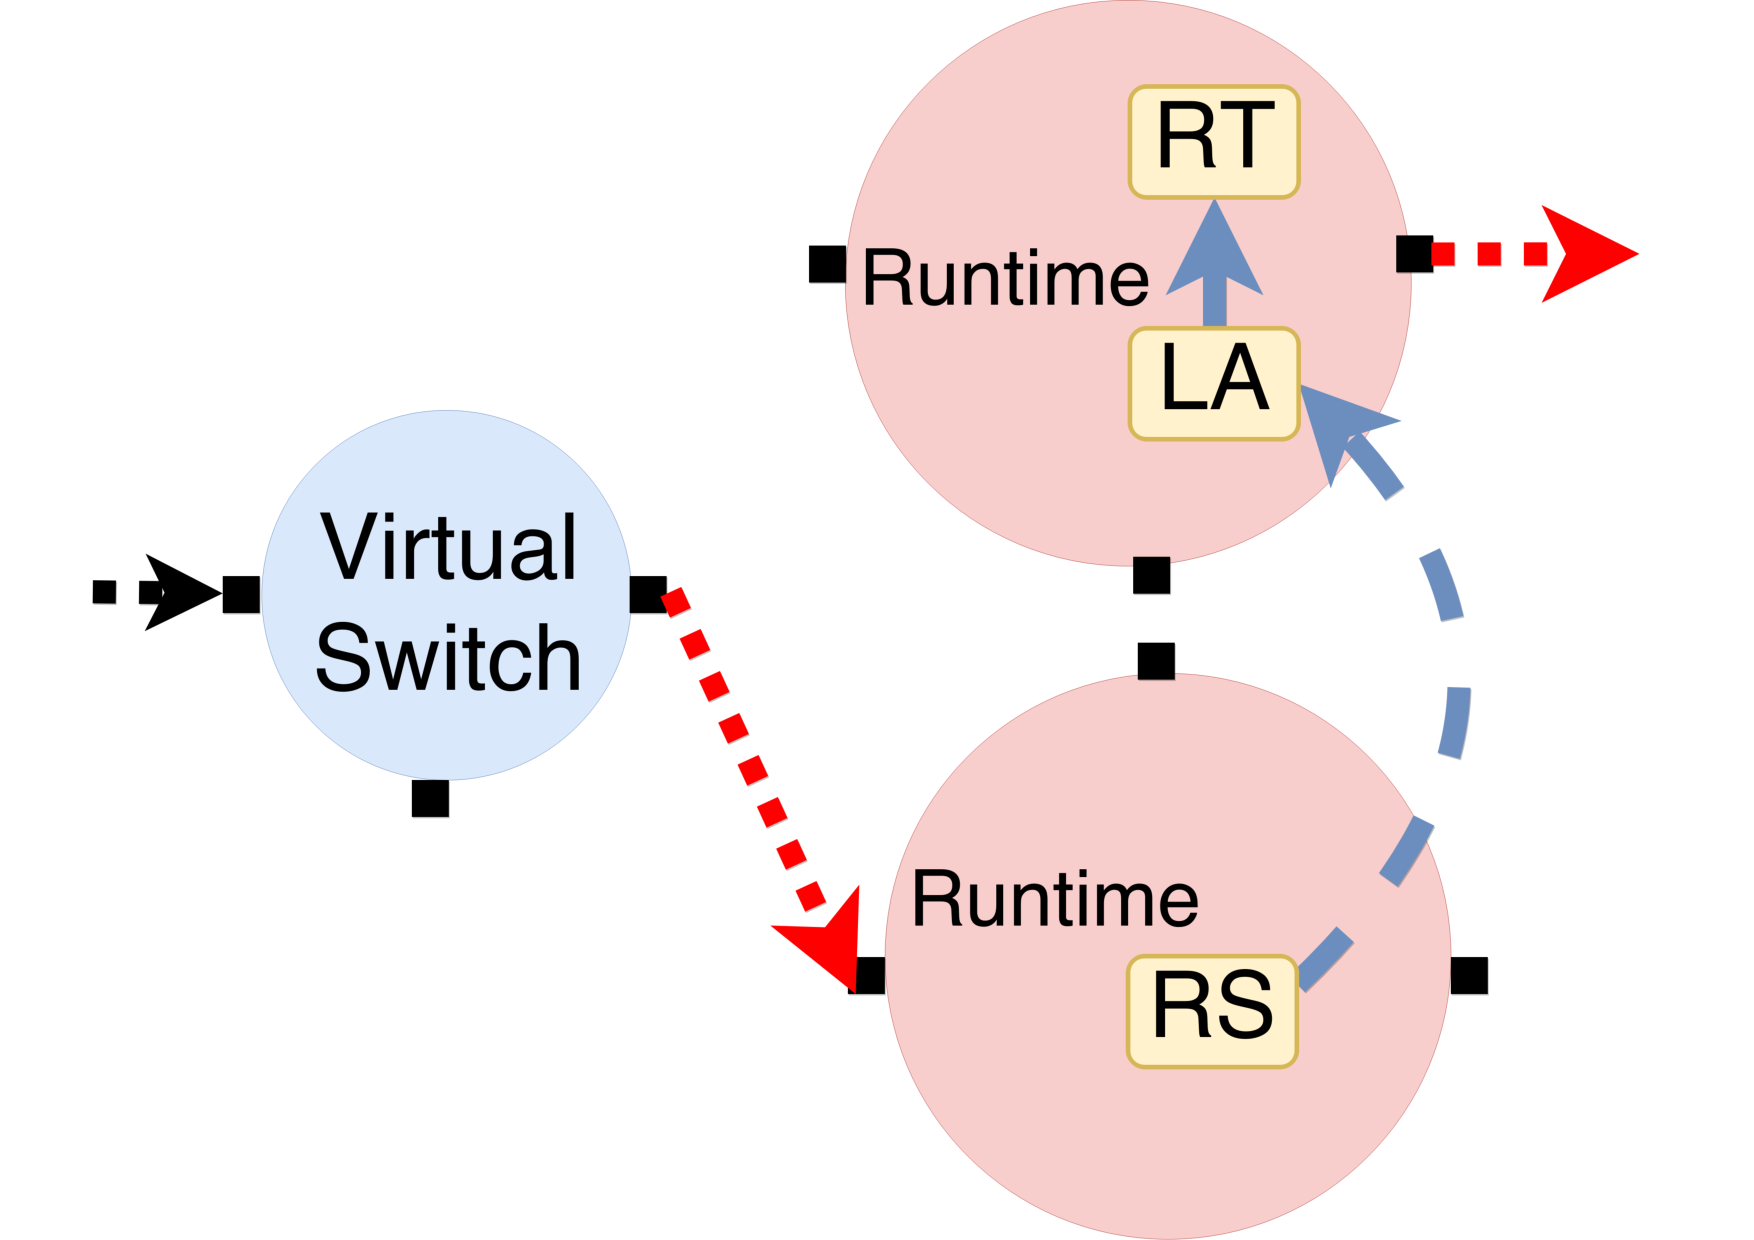
\includegraphics[width=0.66\columnwidth]{figure/nfactor-replication.pdf}
   \caption{Flow replication.}\label{fig:rep}
  \end{subfigure}
  \begin{subfigure}[t]{0.49\linewidth}
     \centering
     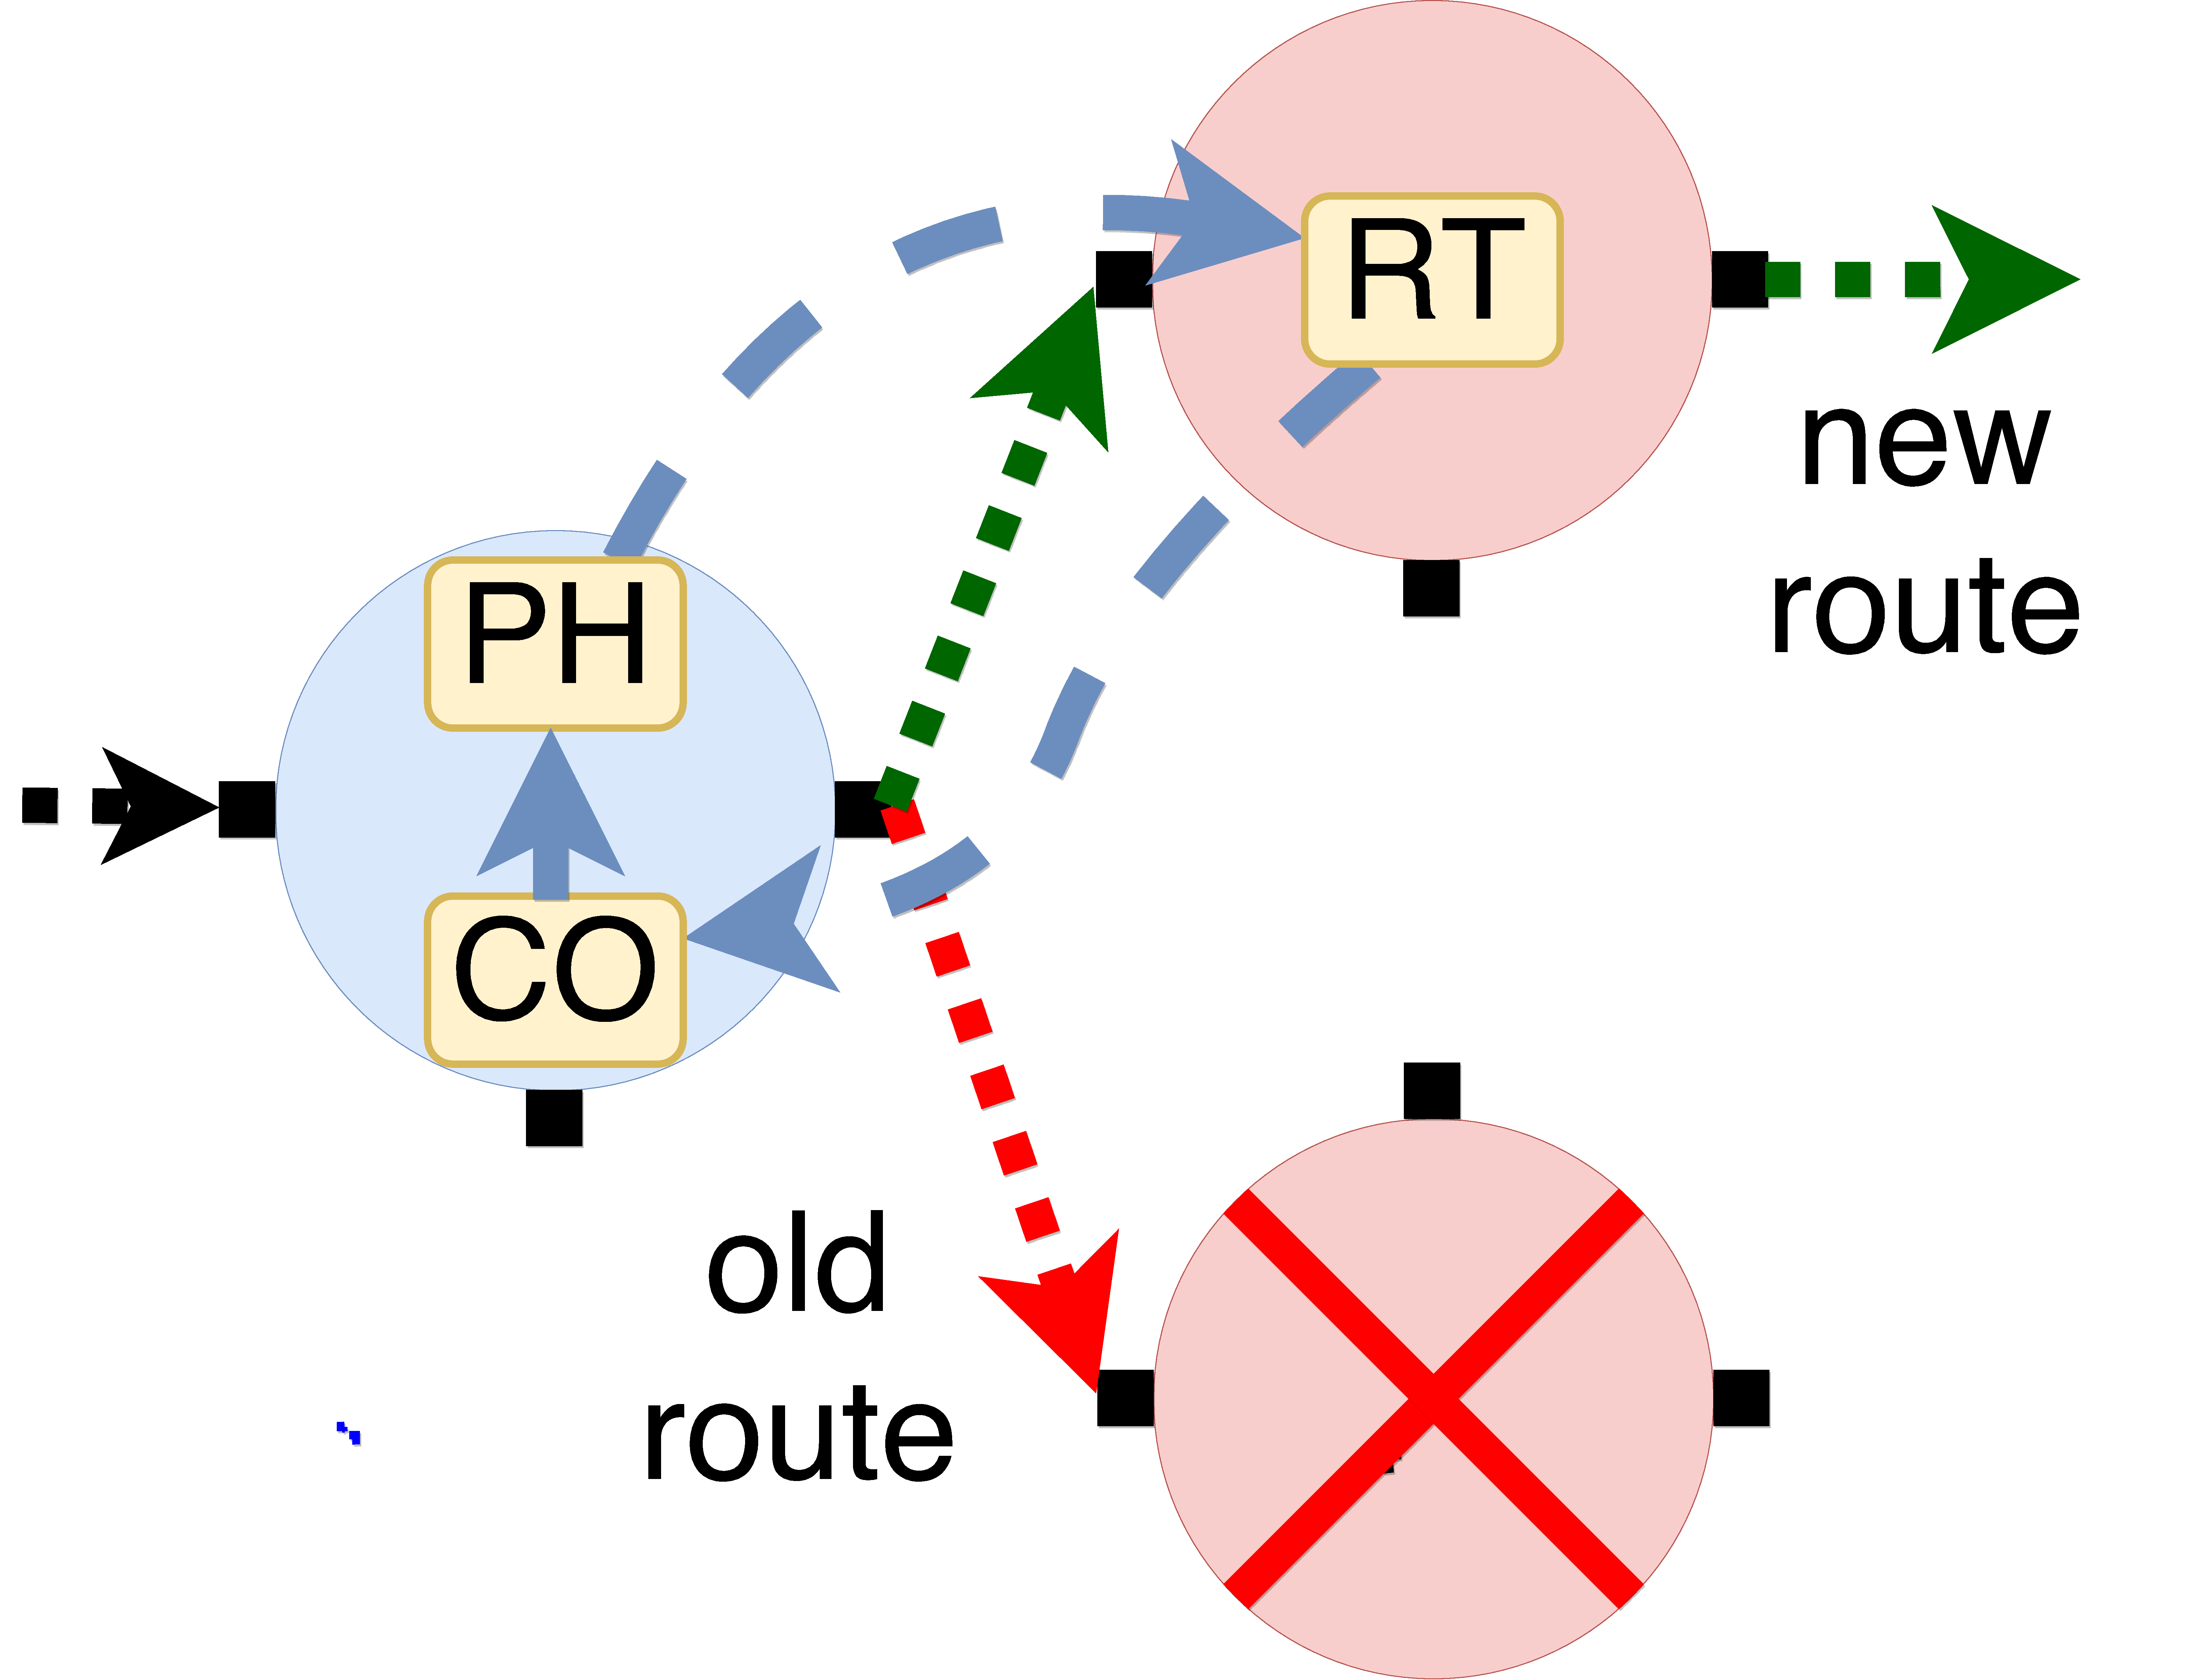
\includegraphics[width=0.66\columnwidth]{figure/nfactor-recover.pdf}
     \caption{Flow recover. The original runtime has failed.}\label{fig:recover}
    \end{subfigure}
 \caption{Flow replication that replicates the original actor running on the original runtime to replica runtime. (\textbf{RT}: Replication target actor. \textbf{RS}: Replication source actor. \textbf{CO}: Coordinator actor. \textbf{VS}: Virtual switch actor. \textbf{Dotted line}: Dataplane flow packets. \textbf{Dashed line}: Actor messages.)}
\label{fig:flow-rep}
\end{figure}

The biggest difference of the \nfactor's replication method and existing works such as \cite{sherry2015rollback} is that NFActor framework replicates individual flow, not NF. This replication strategy is transparent to the NF modules and improves the scalability and resource utilization rate of \nfactor. as flows could be directly replicated on another runtime, without the need for a dedicated backup server. In the mean time, this fine grained replication strategy provides a the same output-commit property as indicated in \cite{sherry2015rollback} with a desirable replication throughput and fast recovery time.

The detailed flow replication process is shown in figure \ref{fig:flow-rep}. When a flow actor is created, it acquires its replica runtime by querying a round-robin list. If the flow actor has a valid replica runtime, whenever it finishes processing the packet, it sends a remote message, containing the current flow state and the packet, to the coordinator actor on the replication target runtime. The coordinator actor on the replication target runtime creates a replica flow actor using the same flow-5-tuple as the original flow actor to handle all the replication messages. The replica flow actor saves the flow state and sends the packet out from the output port of the replica runtime. Similar with \cite{sherry2015rollback}, the receiver on the side of the output port of the replica runtime can only observe an output packet when the flow state has been replicated.

When a runtime fails, the coordinator sends recovery RPC requests \ref{} to all the replica runtime of the failed runtime. This RPC enables replica flow actor to send a request to the virtual switch actor, asking it to change the destination runtime to the replica runtime. When the response is received by the replica flow actor, the original flow is successfully restored on the replica runtime.

